\section{Difficulties with Extreme Class Imbalance}
\label{sec:skew}
Practical applications rarely provide us with data that have equal numbers of training instances of all the classes.  However, in many applications, the imbalance in the distribution of naturally occurring instances is extreme.  For example, when labeling web pages to identify specific content of interest, uninteresting pages may outnumber interesting ones by a million to one or worse (consider identifying web pages containing hate speech, in order to keep advertisers off them, cf.~\cite{attprovkdd2010}).

Prior sections have detailed techniques that have been developed to cope with moderate class imbalance. However, as class imbalances tends towards the extreme, active learning strategies can fail completely--- and this failure is not simply due to the challenges of learning models with skewed class distributions, which has received a good bit of study and has been addressed throughout this book.  The lack of labeled data compounds the problem, because techniques cannot concentrate on the minority instances, as the techniques are unaware which instances to focus on.

Figure~\ref{fig:vary_skew} compares the AUC of logistic regression text classifiers induced by labeled instances selected with uncertainty sampling and with random sampling.  The learning task is to differentiate sports web pages from non-sports pages.  Depending on the source of the data (e.g., different impression streams from different on-line advertisers), one could see very different degrees of class skew in the population of relevant web pages.
The panels in Figure~\ref{fig:vary_skew}, left-to-right, depict increasing amounts of induced class skew.  On the far left, we see that for a balanced class distribution, uncertainty sampling is indeed better than random sampling.  For a 10:1 distribution, uncertainty sampling has some problems very early on, but soon does better than random sampling---even more so than in the balanced case.  However, as the skew begins to get large, not only does random sampling start to fail (it finds fewer and fewer minority instances, and its learning suffers), uncertainty sampling does substantially worse than random for a considerable amount labeling expenditure.  In the most extreme case shown,\footnote{10,000:1 --- still orders of magnitude less skewed than some categories} both random sampling and uncertainty sampling simply fail completely.  Random sampling effectively does not select any positive examples, and neither does uncertainty sampling.\footnote{The curious behavior of AUC$<0.5$ here is due to overfitting.  Regularizing the logistic regression ``fixes'' the problem, and the curve hovers about $0.5$.  See another article in this issue for more insight on models exhibiting AUC$<0.5$~\cite{claudia10xvalid}.}

%We see that as the skew increases, uncertainty sampling and random sampling have increased difficulty selecting minority instances, yielding classifiers with poor generalization performance. In the most skewed setting, random sampling and uncertainty sampling are unable to select reliably \emph{any} minority instances given $10,000$ draws from the available pool.

% It should be noted that while $10,000$ to $1$ may be an extremely skewed class distribution for the active learning literature, far greater skews are faced in practice, particularly when performing classification on the web.

A practitioner well-versed in the active learning literature may decide she should use a method other than uncertainty sampling in such a highly skewed domain.  A variety of techniques have been discussed in Sections~\ref{sec:related},~\ref{al_for_imbalanced_data}, and~\ref{virtual} for performing active learning specifically under class imbalance, including~\cite{tomanek2009imbalance, bloodgood2009imbalance, zhu2007imbalance, Ertekin2_2007, he2007rarecategory}, as well as for performing density-sensitive active learning, where the geometry of the problem space is specifically included when making selections, including~\cite{zhuDensity2008, donmez2008psd, nguyen2004preclustering, xu03representitive, cmccallum98em}. While initially appealing, as problems become increasingly difficult, these techniques may not provide results better than more traditional active learning techniques---indeed class skews may be sufficiently high as to thwart these techniques completely~\cite{attprovkdd2010}.

\begin{figure*}[t!]
\center{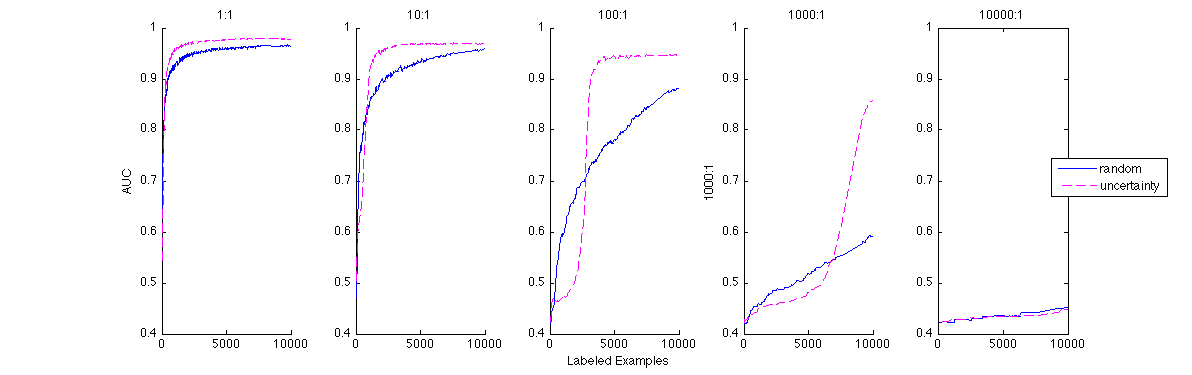
\includegraphics[width=\columnwidth]{plots/varySkewRandUnc2.png}}
\caption{Comparison of random sampling and uncertainty sampling on the same data set with induced skews ranging from $1:1$ to $10,000:1$.}
\label{fig:vary_skew}
\end{figure*}

As discussed later in Section~\ref{sec:acs}, Attenberg and Provost~\cite{attprovkdd2010} proposed an alternative way of using human resources to produce labeled training set, specifically tasking people with finding class-specific instances (``guided learning'') as opposed to labeling specific instances.  In some domains, finding such instances may even be cheaper than labeling (per instance).  Guided learning can be much more effective per instance acquired; in one of Attenberg and Provost's experiments it outperformed active learning as long as searching for class-specific instances was less than eight times more expensive (per instance) than labeling selected instances.  The generalization performance
of guided learning is shown in Figure~\ref{fig:guidedvary_skew}, discussed below in Section~\ref{sec:acs} for the same setting as Figure~\ref{fig:vary_skew}.

\section{Dealing with disjunctive classes}
\label{sec:disjunct}
Even more subtly still, certain problem spaces may not have such an extreme class skew, but may still be particularly difficult because they possess important but very small disjunctive sub-concepts, rather than simple continuously dense regions of minority and majority instances.
Prior research has shown that such ``small disjuncts'' can comprise a large portion of a target class in some domains \cite{WeissAIS2020}.
%Gary M. Weiss (2010). The Impact of Small Disjuncts on Classifier Learning. %Annals of Information Systems, 8:193-226.
For active learning, these small subconcepts act like rare classes: if a learner has seen no instances of the subconcept, how can it ``know'' which instances to label? Note that this is not simply a problem of using the wrong loss function: in an active learning setting, the learner does not even know that the instances of the subconcept are misclassified if no instances of a subconcept have yet been labeled. Nonetheless, in a research setting (where we know all the labels) using an undiscriminative loss function, such as classification accuracy or even the area under the ROC curve (AUC), may result in the researcher not even realizing that an important subconcept has been missed.

To demonstrate how small disjuncts influence (active) model learning, consider the following text classification problem: separating the \emph{science} articles from the \emph{non-science} articles within a subset of the $20$ Newsgroups benchmark set (with an induced class skew of $80$ to $1$).  Figure~\ref{fig:minoritypos} examines graphically the relative positions of the minority instances through the active learning. The black curve shows the AUC (right vertical axis) of the models learned by a logistic regression classifier using uncertainty sampling, rescaled as follows. At each epoch we sort all instances by their predicted probability of membership in the majority class, $\hat{P}(y = 0 | x)$. The blue dots in Figure~\ref{fig:minoritypos} represent the minority class instances, with the value on the left vertical axis showing their relative position in this sorted list. The x-axis shows the active learning epoch (here each epoch requests $30$ new instances from the pool). The blue trajectories mostly show instances' relative positions changing. Minority instances drop down to the very bottom (certain minority) either because they get chosen for labeling, or because labeling some other instance caused the model to ``realize'' that they are minority instances.

\begin{figure}[h!]
\center{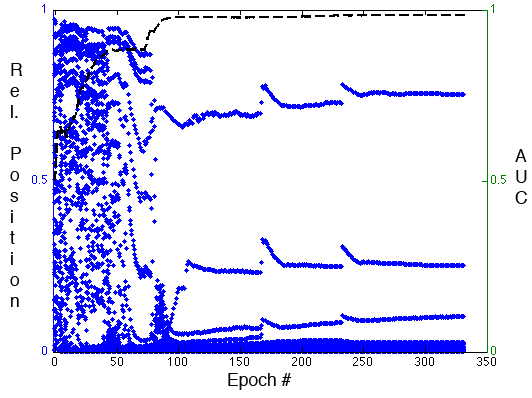
\includegraphics[width=0.8\columnwidth]{plots/position_of_positive_instances_by_p_plus_uncert_feb5.png}}
\caption{A comparison of the learned model's ordering of the instance
  pool, along with the quality of the cross-validated AUC.}
\label{fig:minoritypos}
\end{figure}

We see that, early on, the minority instances are mixed all throughout the range of estimated probabilities, even as the generalization accuracy increases.  Then the model becomes good enough that, abruptly, few minority class instances are misclassified (above $\hat{P}=0.5$).  This is the point where the learning curve levels off for the first time.  However, notice that there still are some residual misclassified minority instances, and in particular that there is a cluster of them for which the model is relatively certain they are \emph{majority} instances.  It takes many epochs for the active learning to select one of these, at which point the generalization performance increases markedly---apparently, this was a subconcept that was strongly misclassified by the model, and so it was not a high priority for exploration by the active learning.

On the $20$ Newsgroups data set we can examine the minority instances for which $\hat{P}$ decreases the most in that late rise in the AUC curve (roughly, they \emph{switch} from being misclassified on the lower plateau to being correctly classified afterward).  Recall that the minority (positive) class here is ``Science'' newsgroups.  It turns out that these late-switching instances are members of the cryptography (sci.crpyt) subcategory.  These pages were classified as non-Science presumably because before having seen any positive instances of the subcategory, they looked much more like the many computer-oriented subcategories in the (much more prevalent) non-Science category.  As soon as a few were labeled as Science, the model generalized its notion of Science to include this subcategory (apparently pretty well).

Density-sensitive active learning techniques did not improve upon uncertainty sampling for this particular domain.  This was surprising, given the support we have just provided for our intuition that the concepts are disjunctive. One would expect a density-oriented technique to be appropriate for this domain.  Unfortunately in this domain---and we conjecture that this is typical of many domains with extreme class imbalance---the \emph{majority} class is \emph{even more disjunctive} than the minority class.  For example, in $20$ Newsgroups, Science indeed has four very different subclasses.  However, non-Science has 16 (with much more variety).  Techniques that (for example) try to find as-of-yet unexplored clusters in the instance space are likely to select from the vast and varied majority class.  We need more research on dealing with highly disjunctive classes, especially when the less interesting\footnote{How interesting a class is could be measured by its relative misclassification cost, for example.} class is more varied than the main class of interest.
